\documentclass{report}
\usepackage[utf8]{inputenc}
\usepackage{amsmath}
\usepackage{graphicx}
\usepackage{pdfpages}
\usepackage{listings}
\usepackage{fancyhdr}
\usepackage{import}

\title{MATH 316 Notes}
\author{Ashtan Mistal}
\date{May - June 2021}

\pagestyle{fancy}
\fancyhf{}
\rhead{Lecture \thechapter}
\lhead{MATH 316 Notes}
\rfoot{Page \thepage}

\begin{document}

\maketitle

\tableofcontents{}

\chapter{Lecture 1}
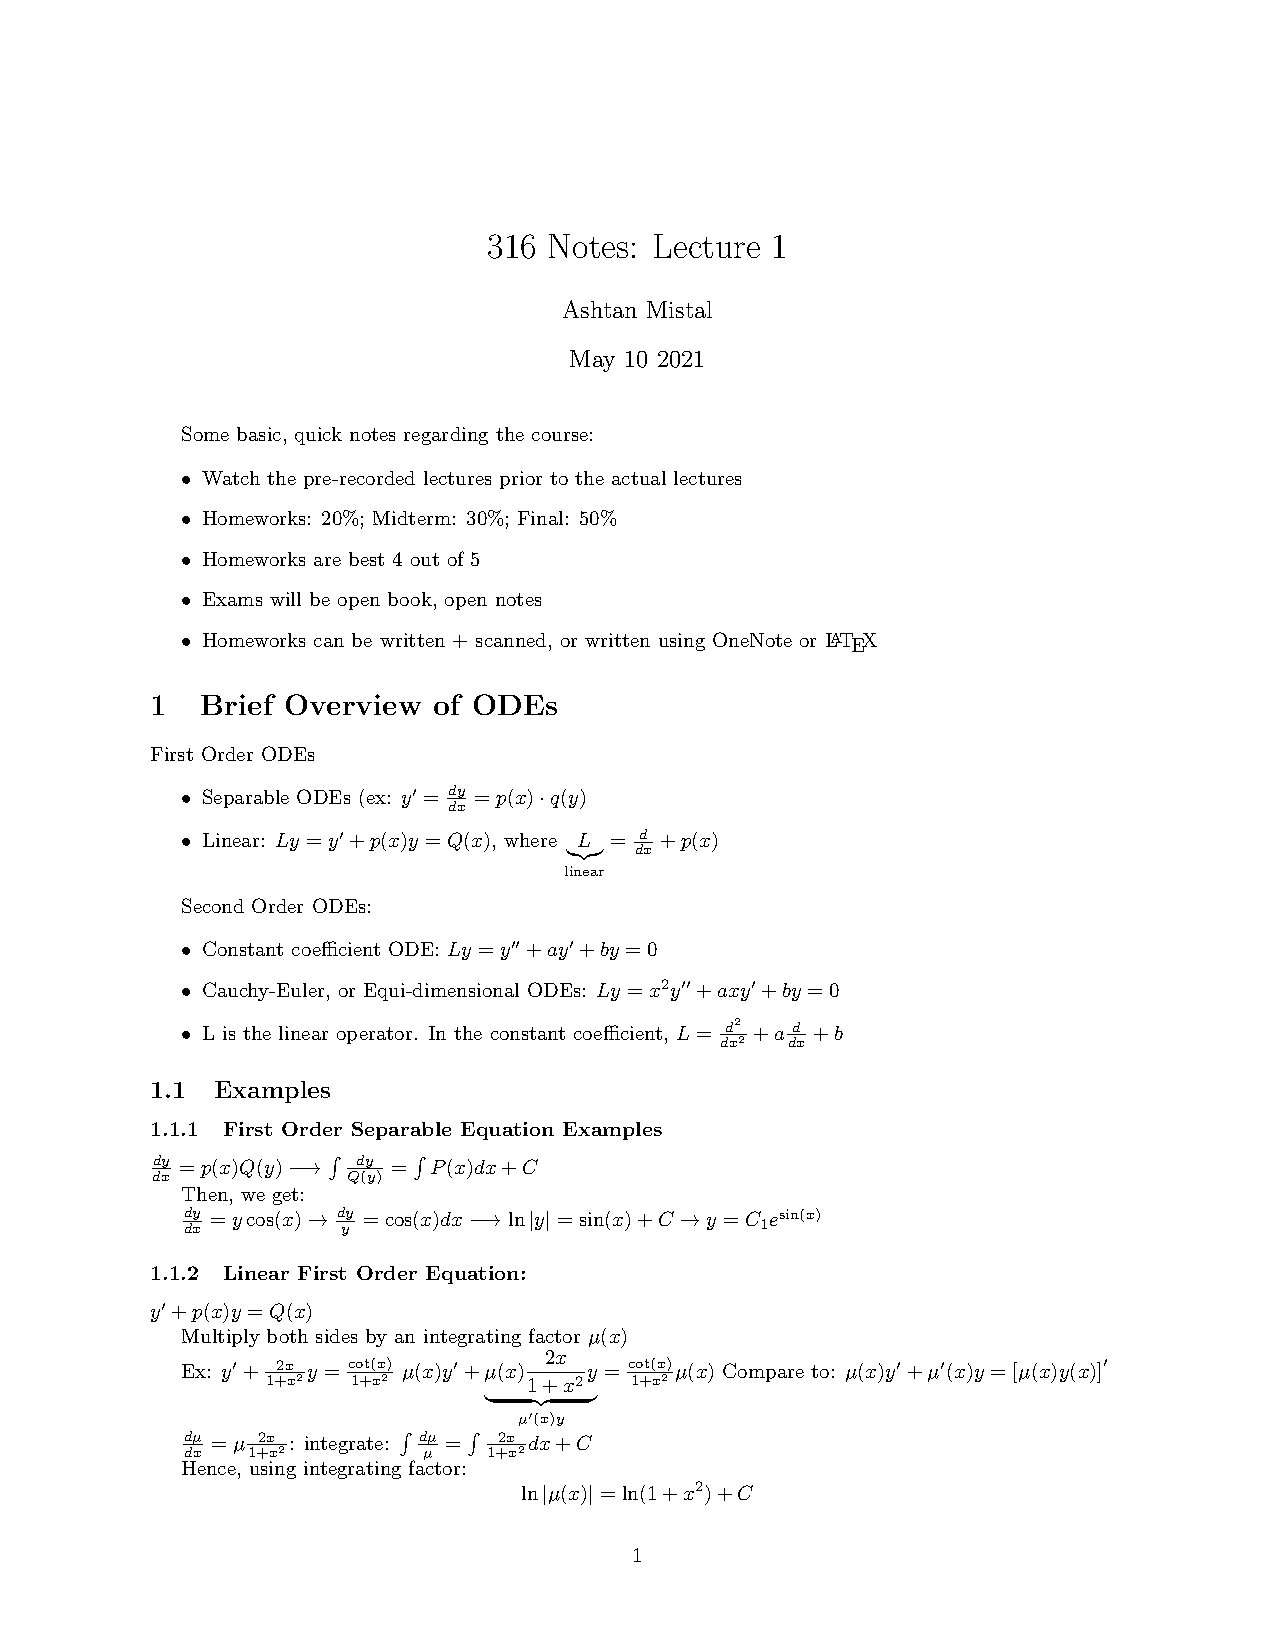
\includepdf[pages=-]{MATH 316 Lecture 1.pdf}

\chapter{Lecture 2}
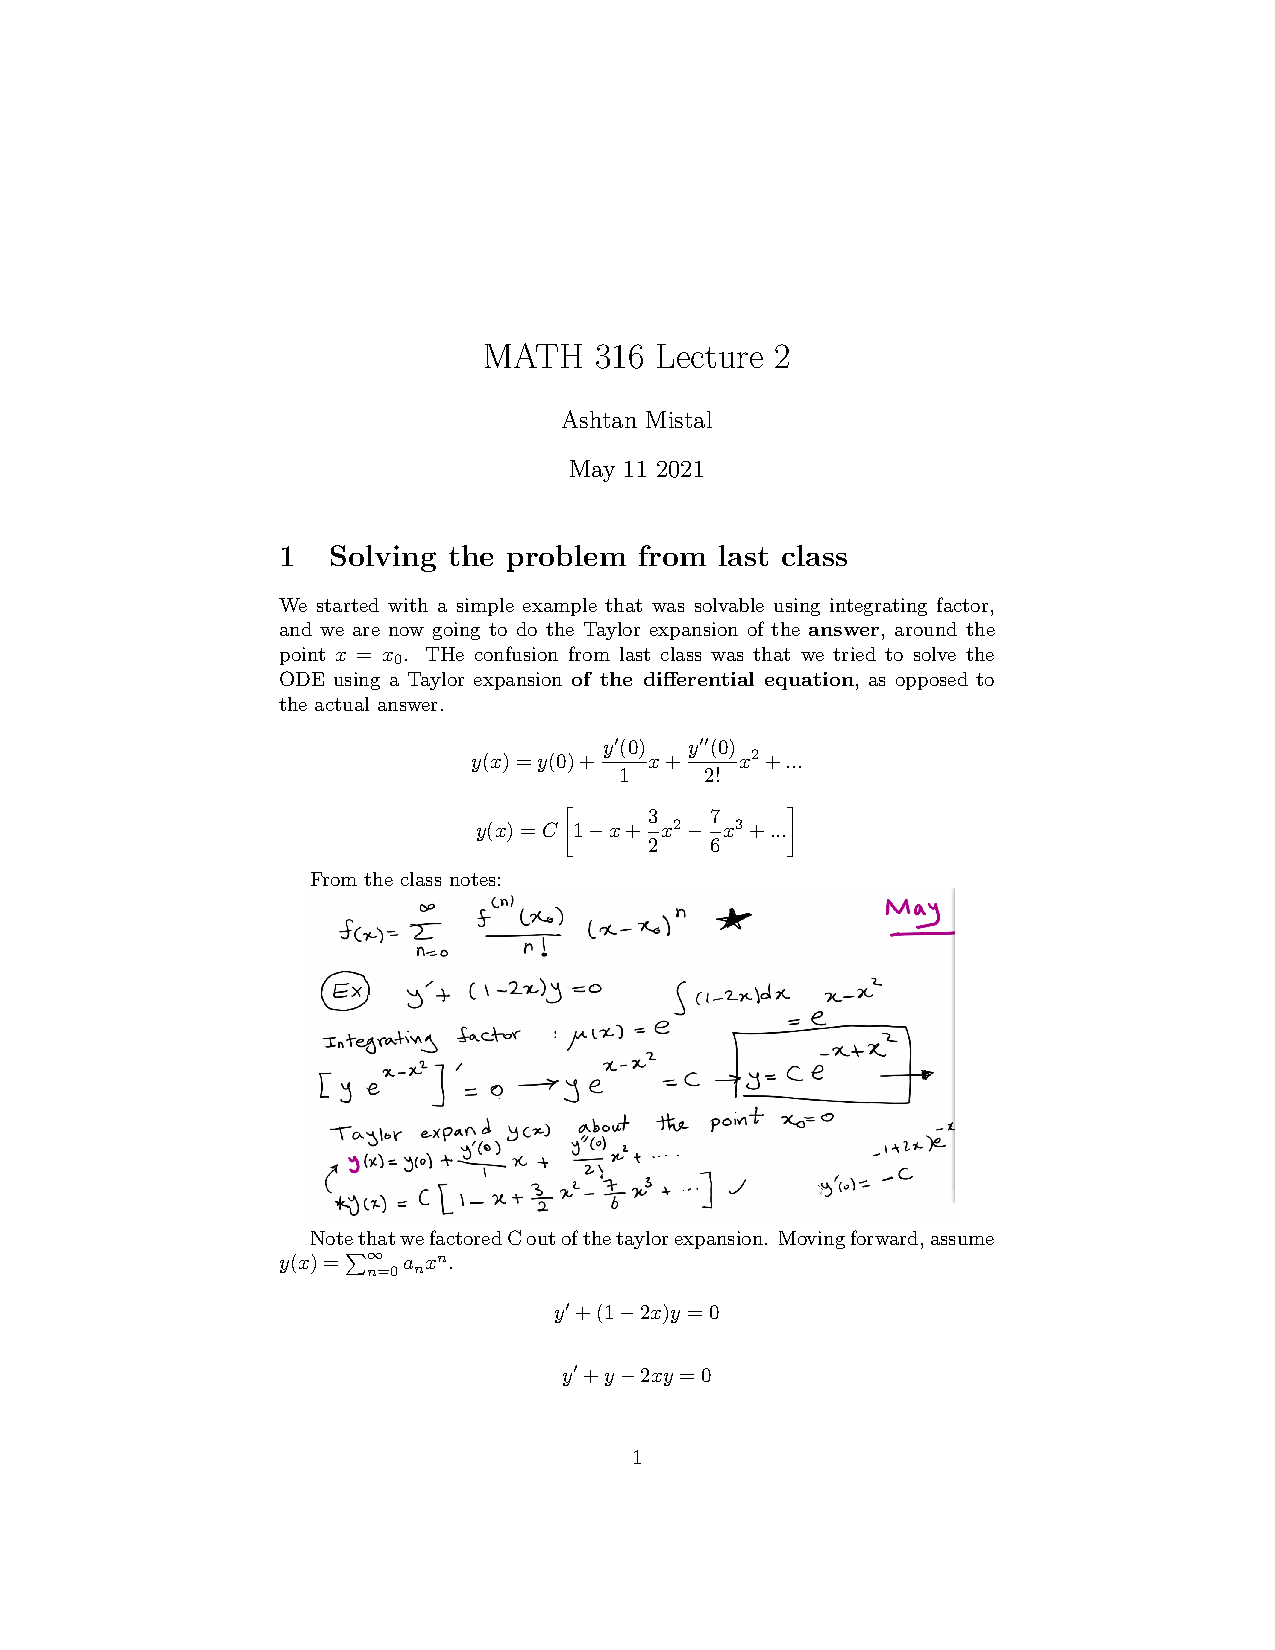
\includepdf[pages=-]{MATH 316 Lecture 2.pdf}

\chapter{Lecture 3}
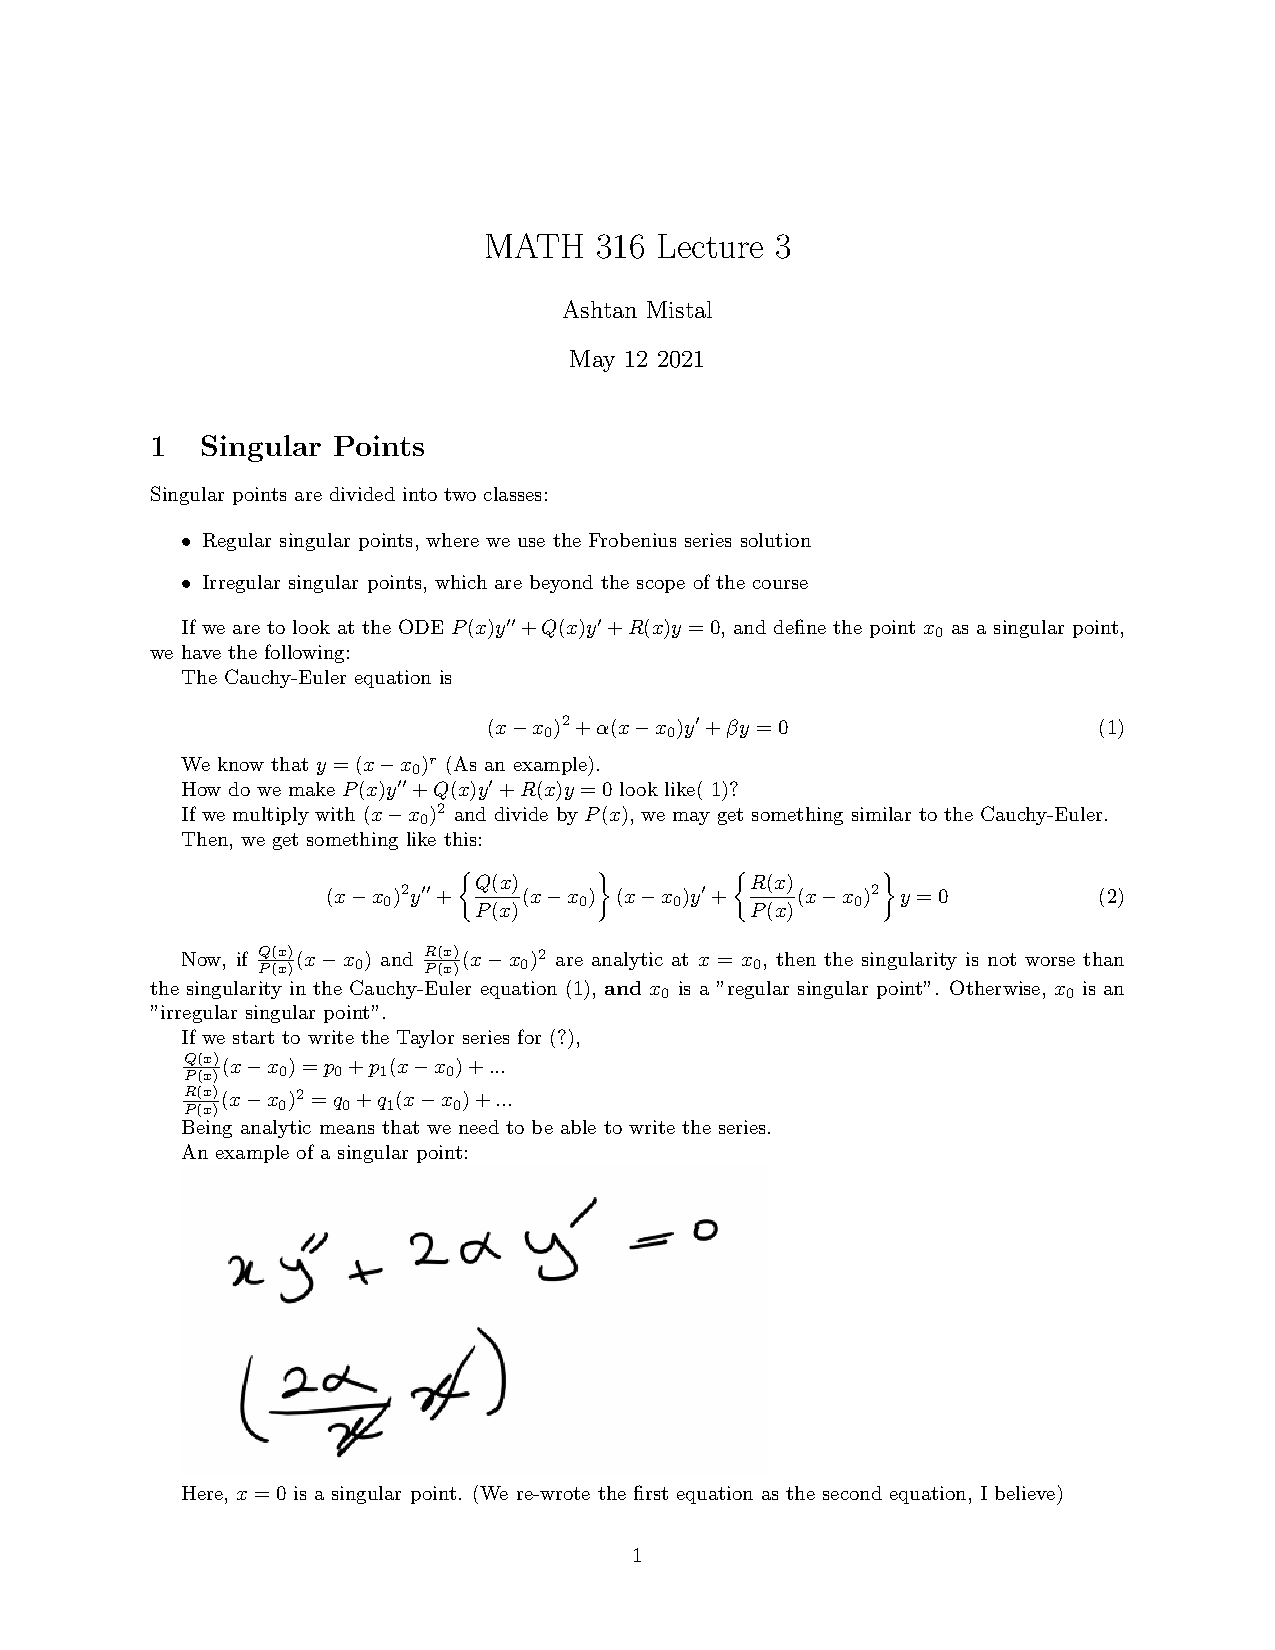
\includepdf[pages=-]{MATH 316 Lecture 3.pdf}

\chapter{Lecture 4}
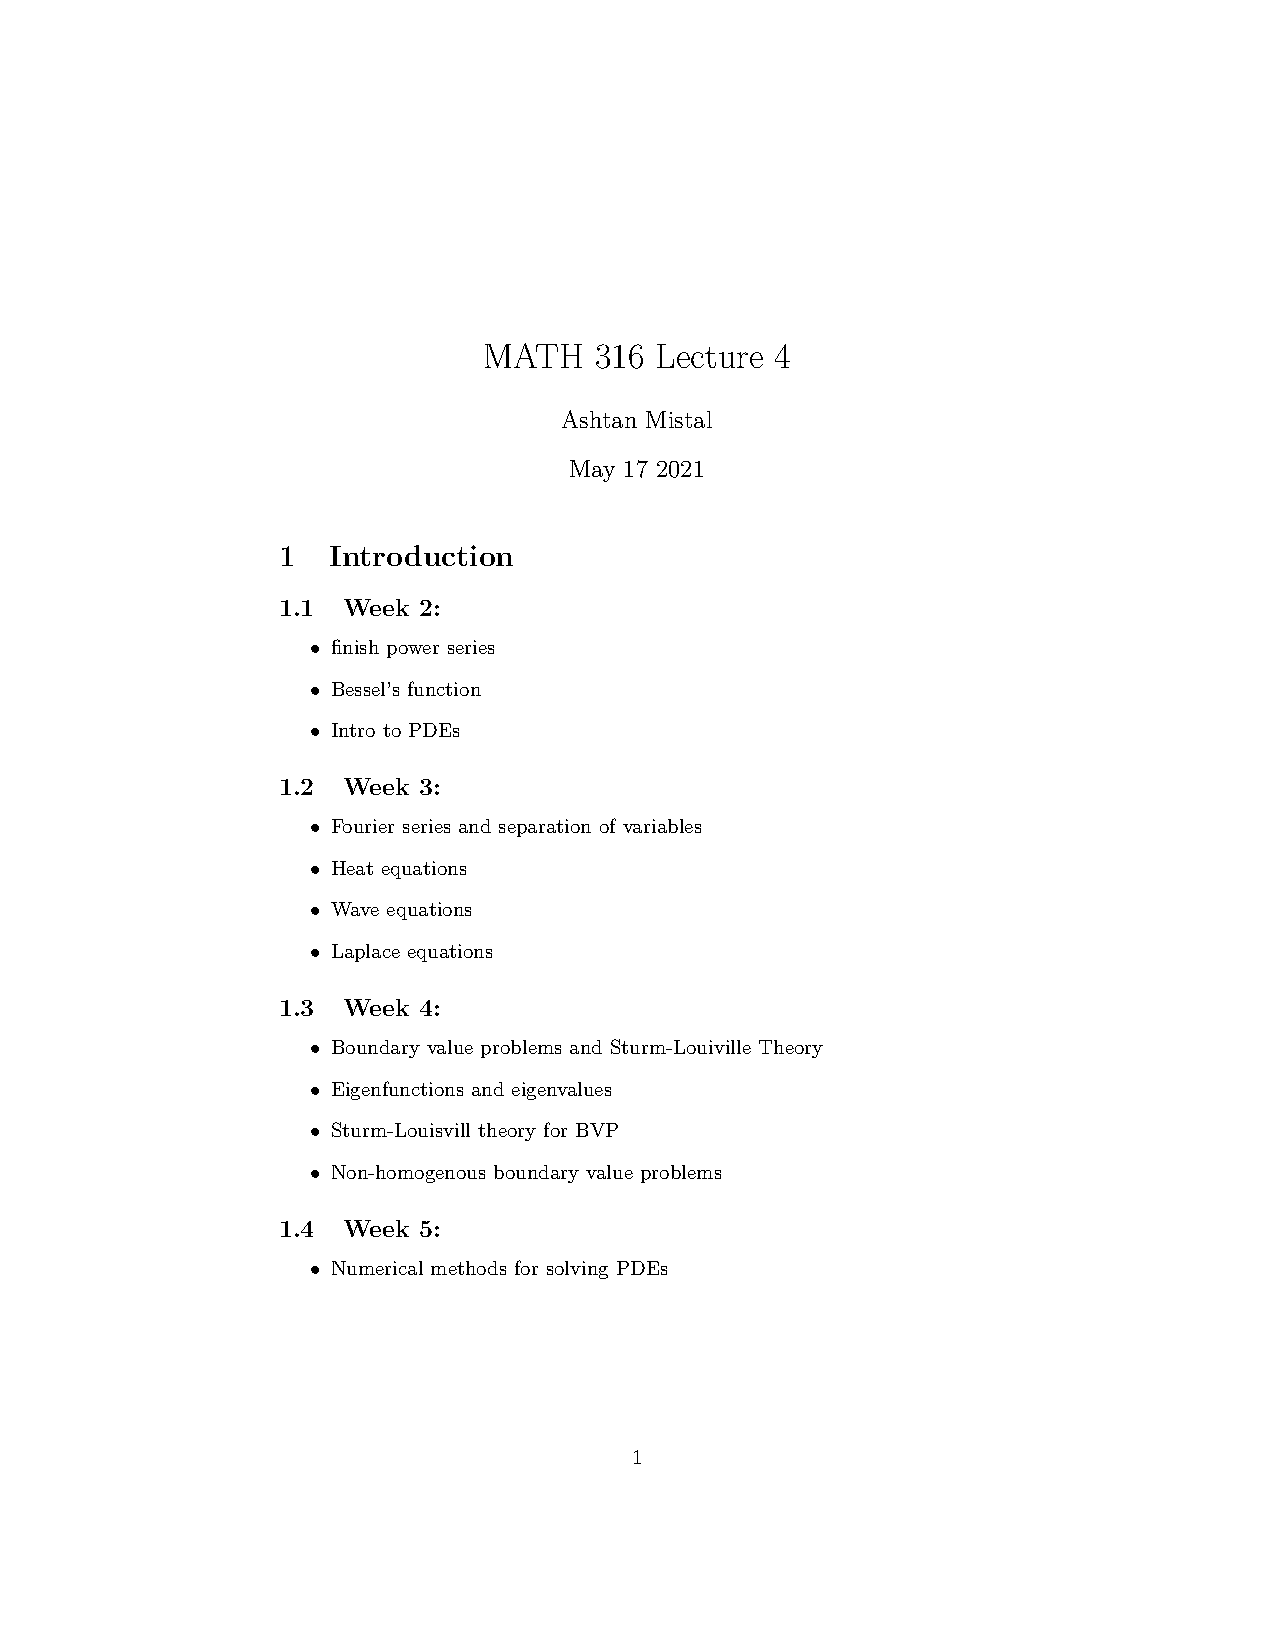
\includepdf[pages=-]{MATH 316 Lecture 4.pdf}

\chapter{Lecture 5}
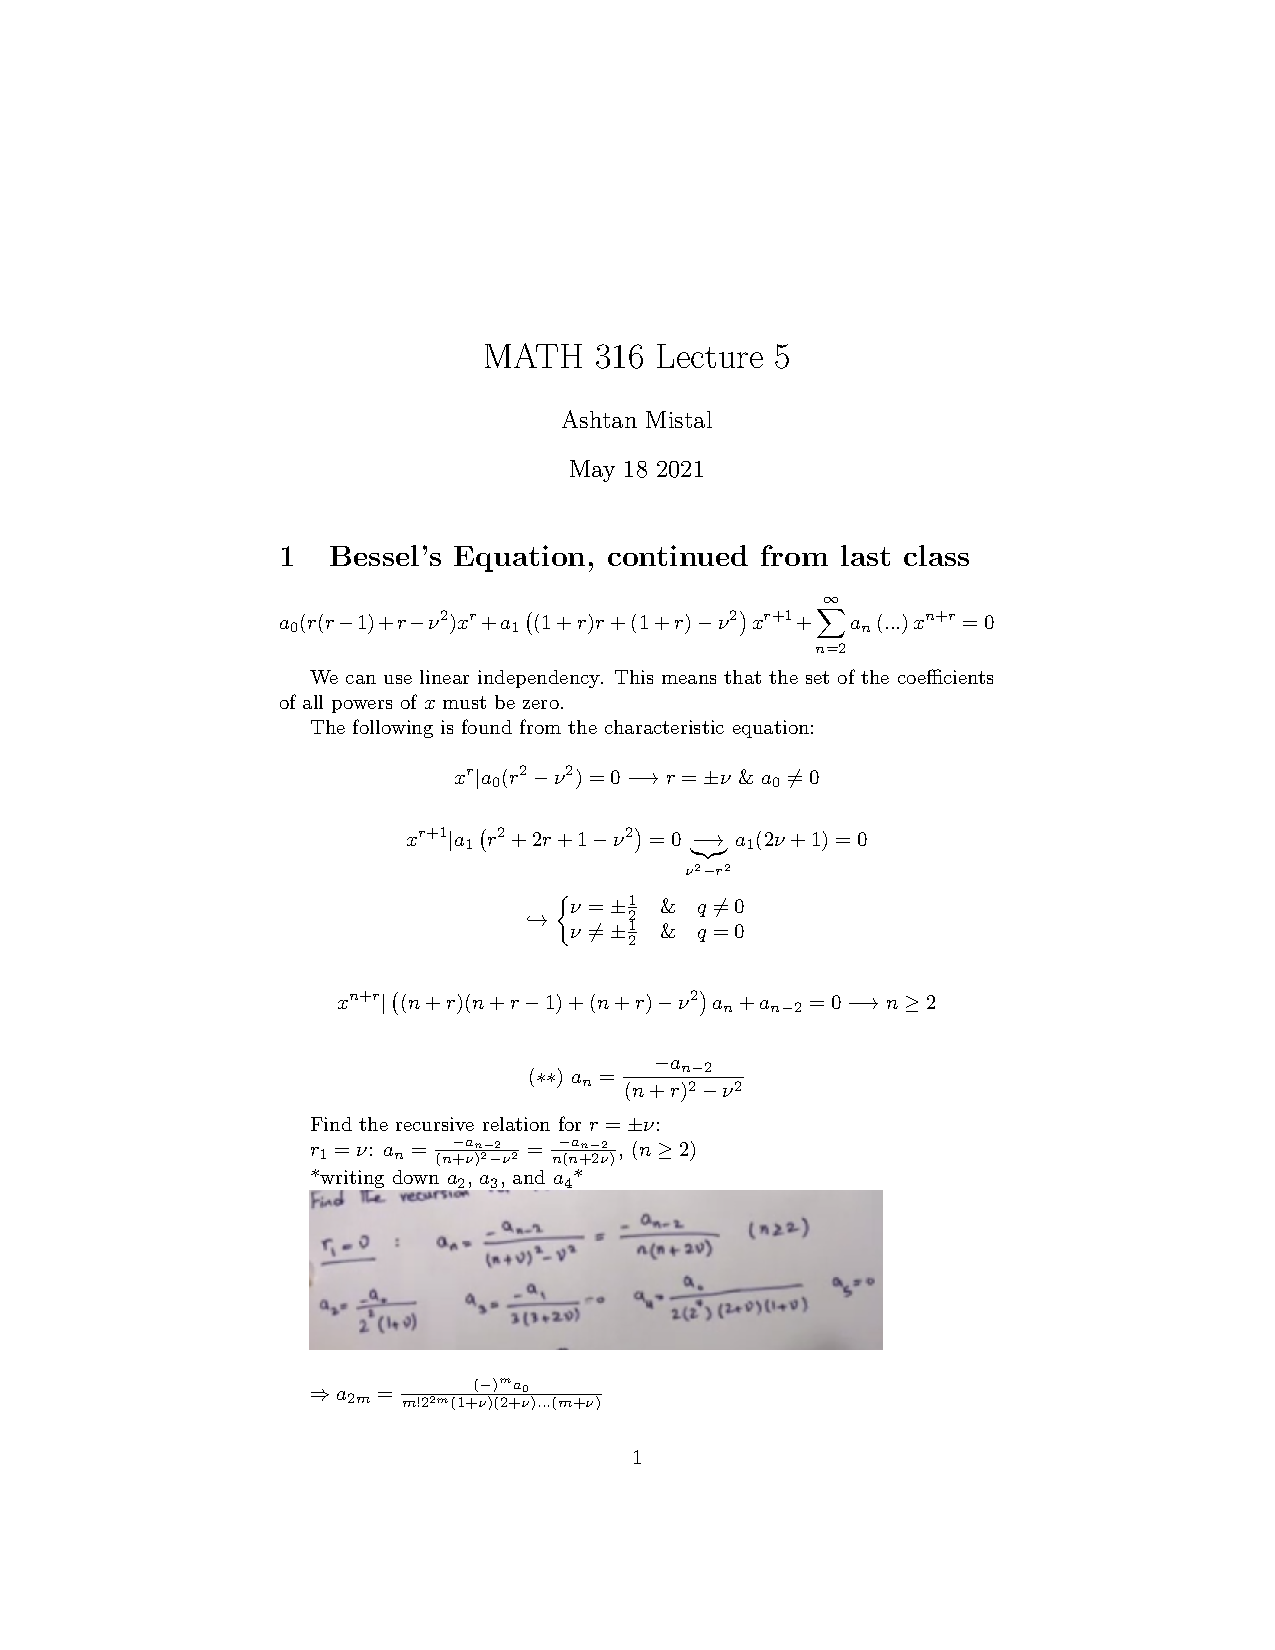
\includepdf[pages=-]{MATH 316 Lecture 5.pdf}

\chapter{Lecture 6}
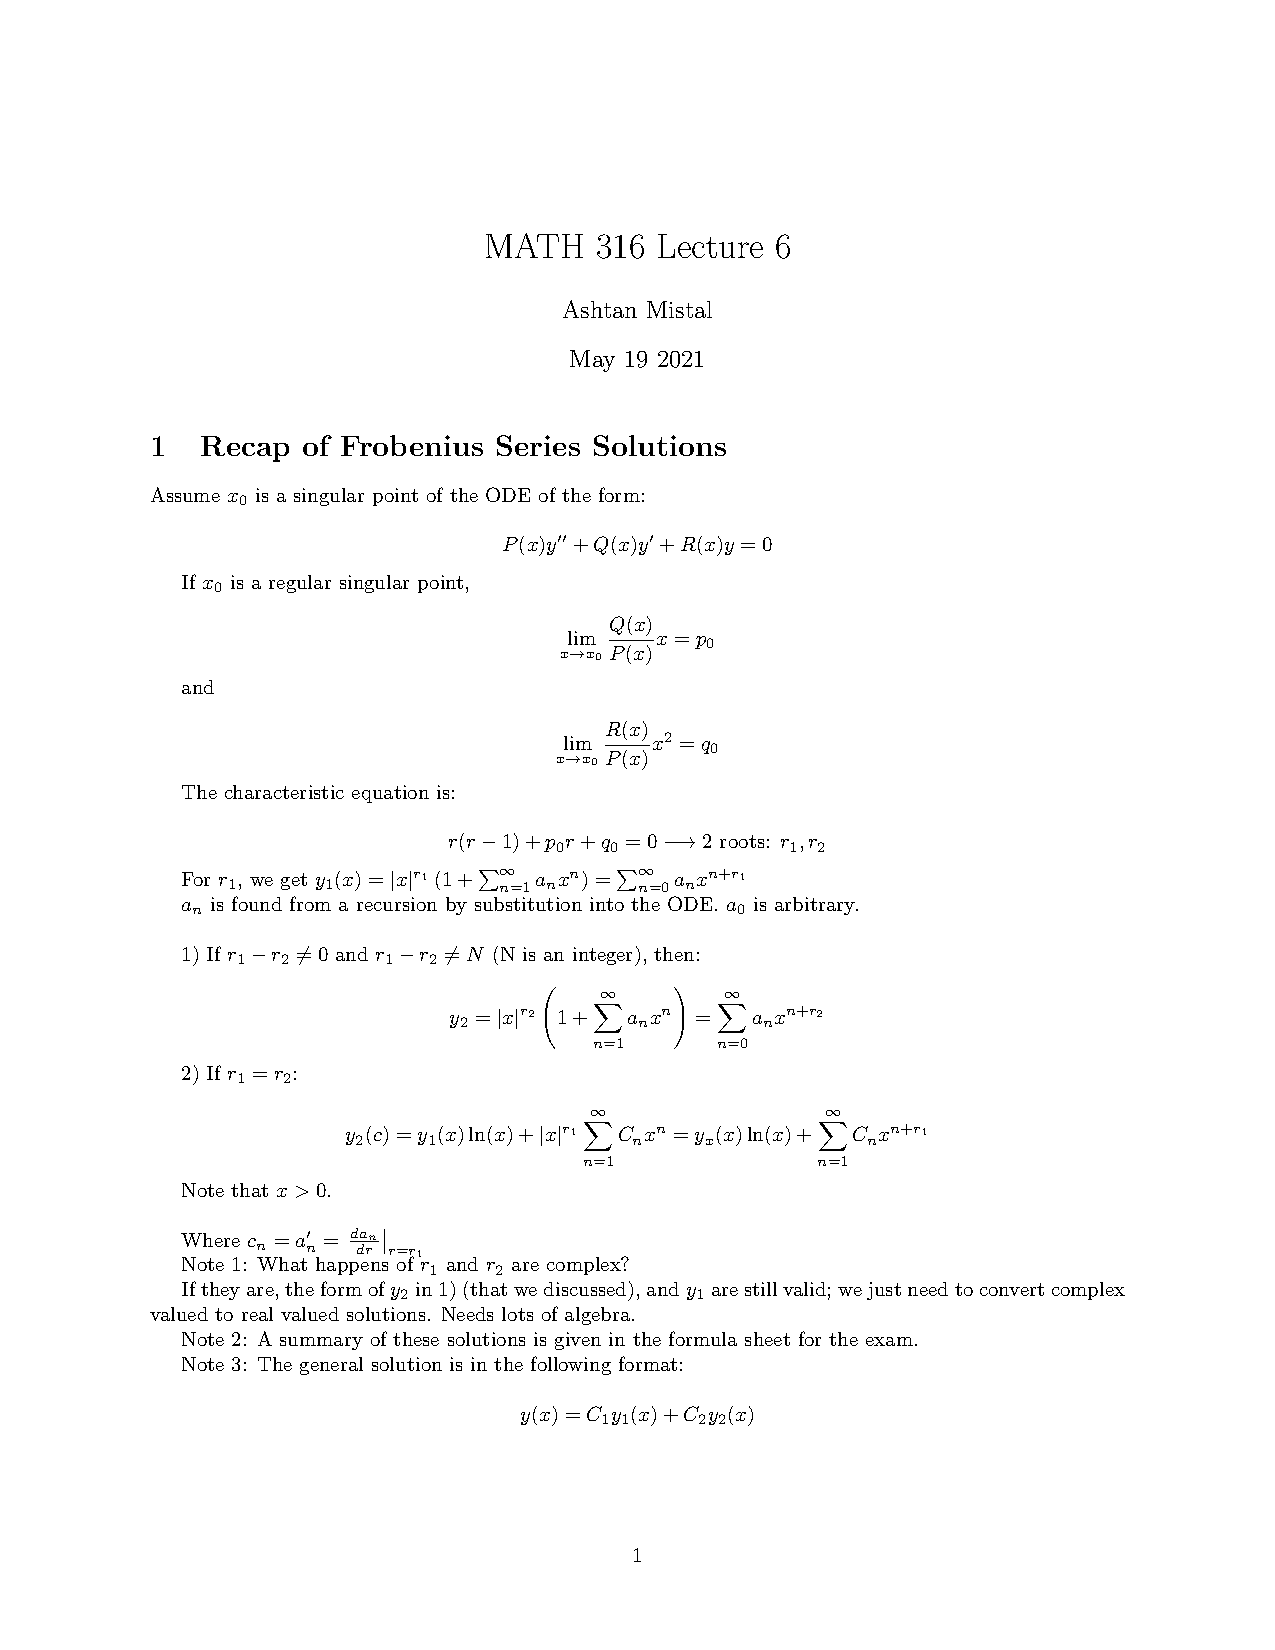
\includepdf[pages=-]{MATH 316 Lecture 6.pdf}

\chapter{Lecture 7}
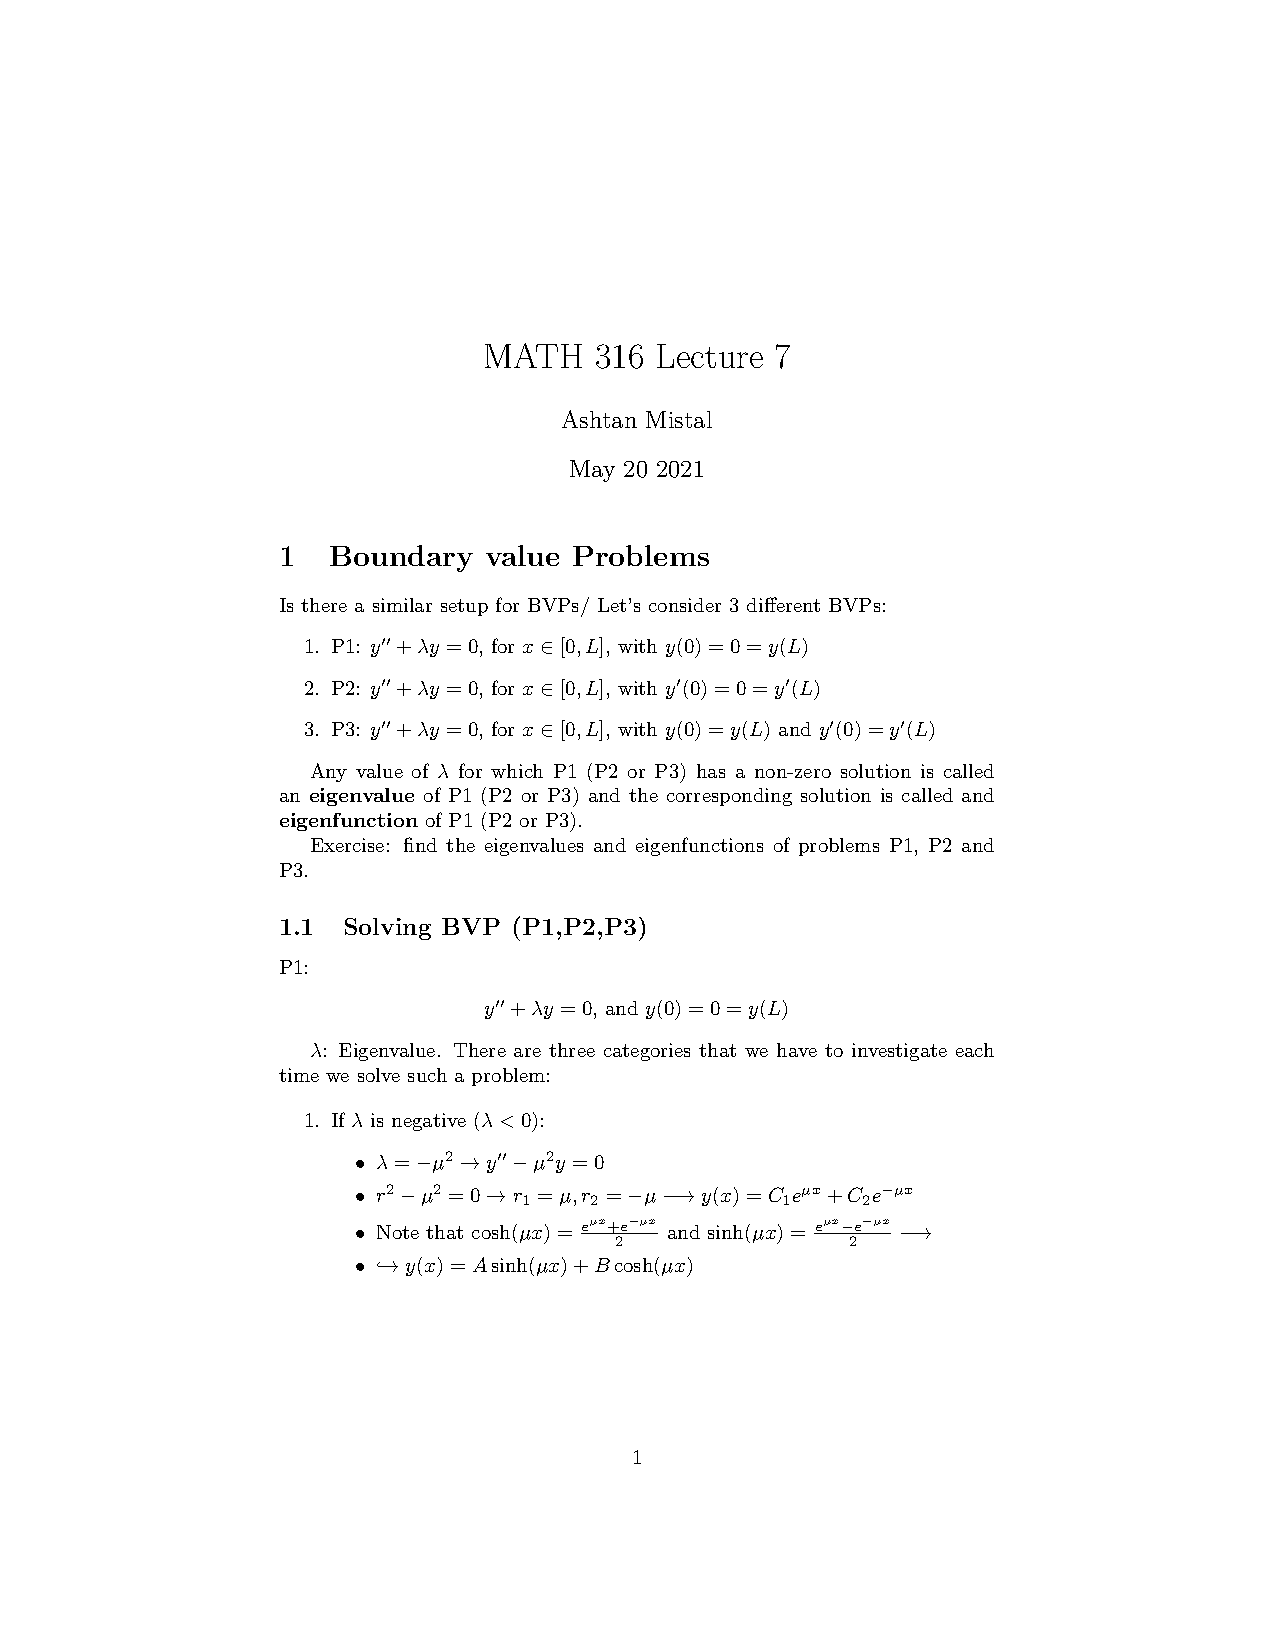
\includepdf[pages=-]{MATH 316 Lecture 7.pdf}

\chapter{Lecture 8}
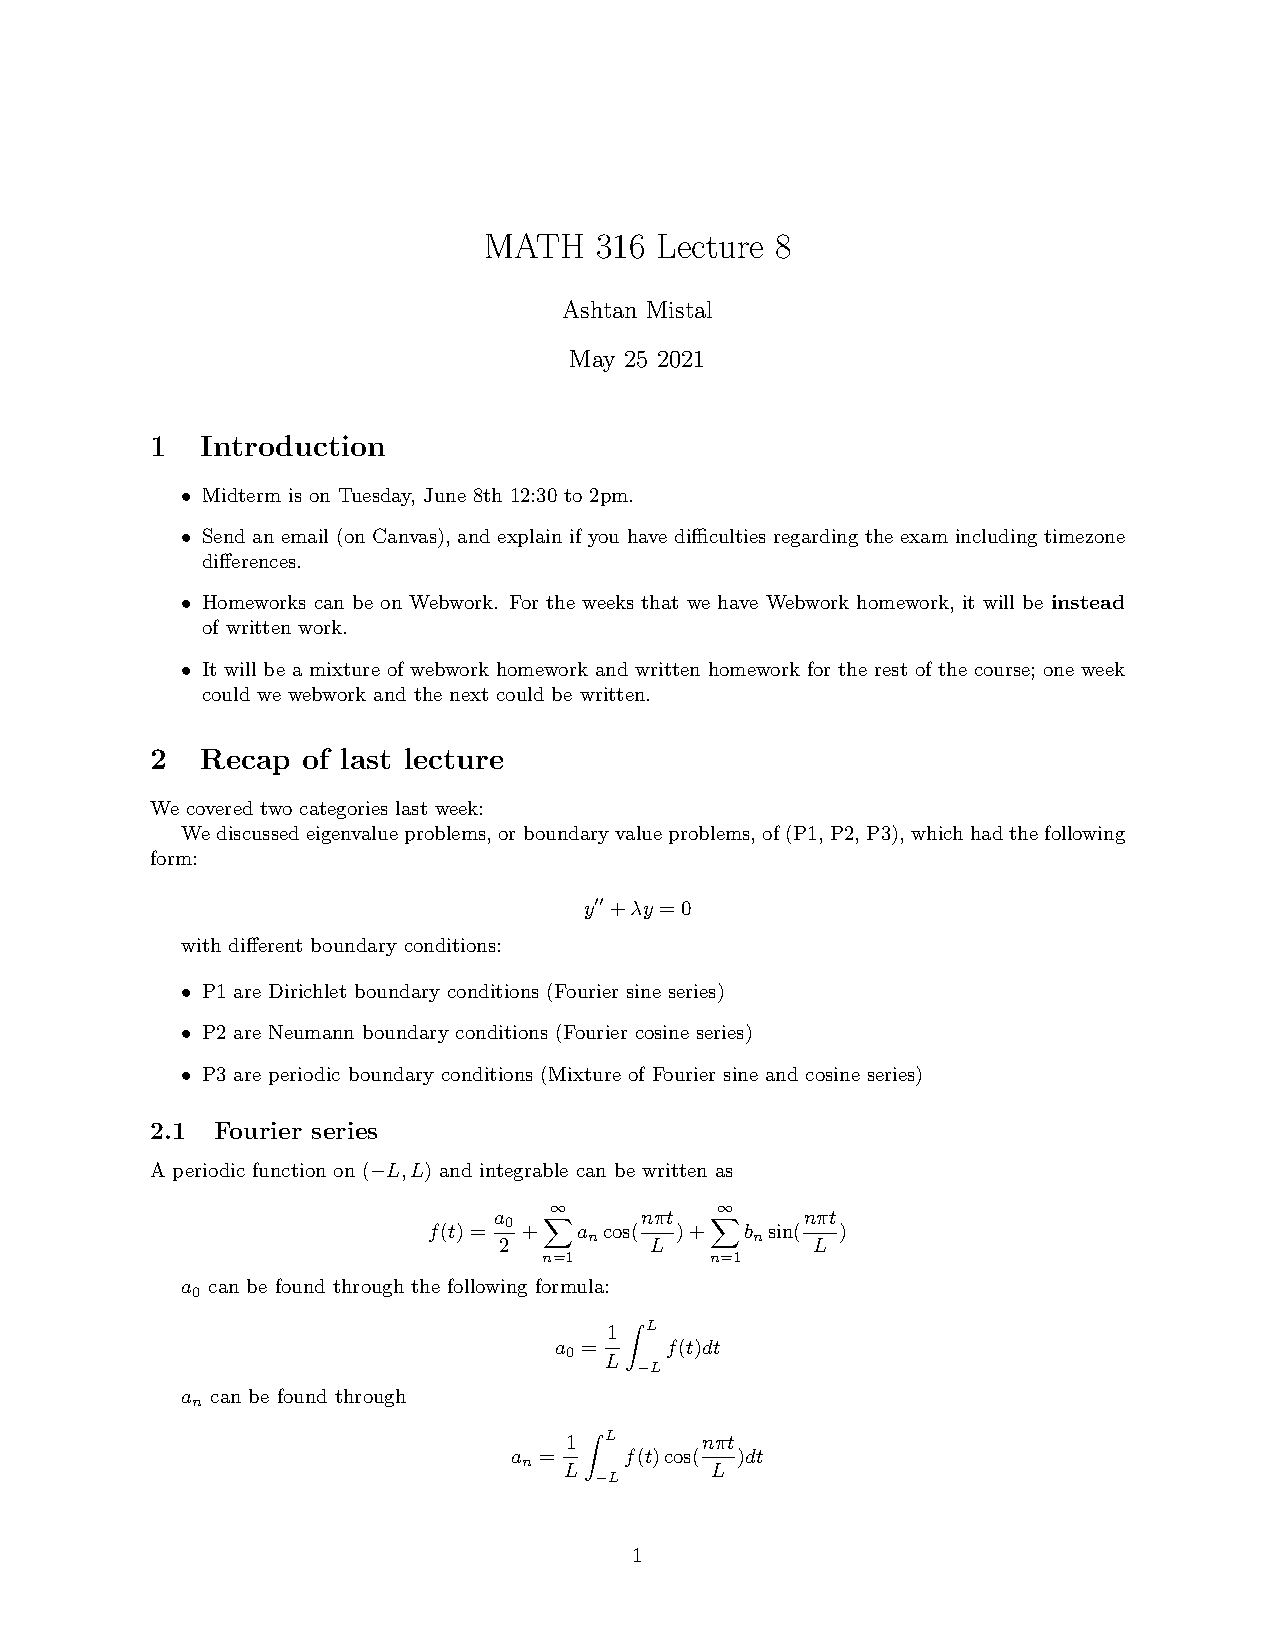
\includepdf[pages=-]{MATH 316 Lecture 8.pdf}

\chapter{Lecture 9}
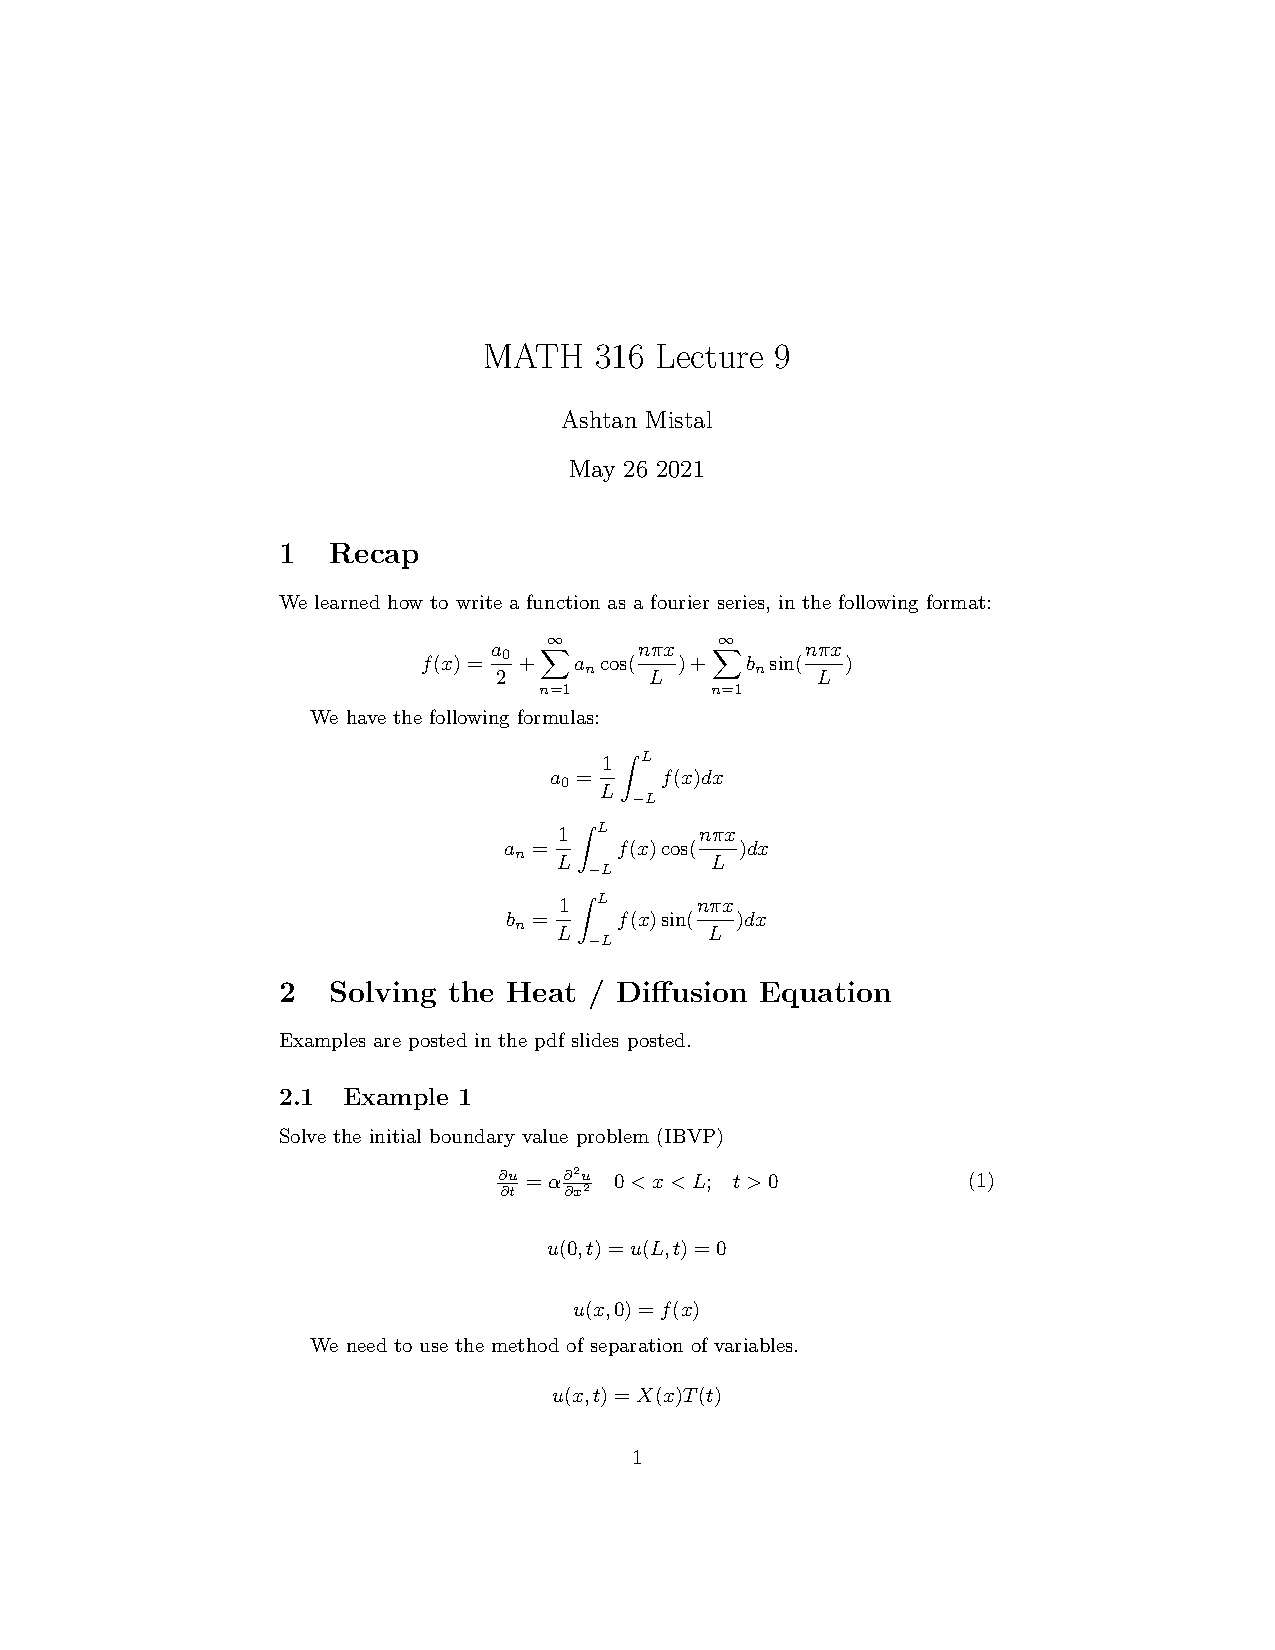
\includepdf[pages=-]{MATH 316 Lecture 9.pdf}

\chapter{Lecture 10}
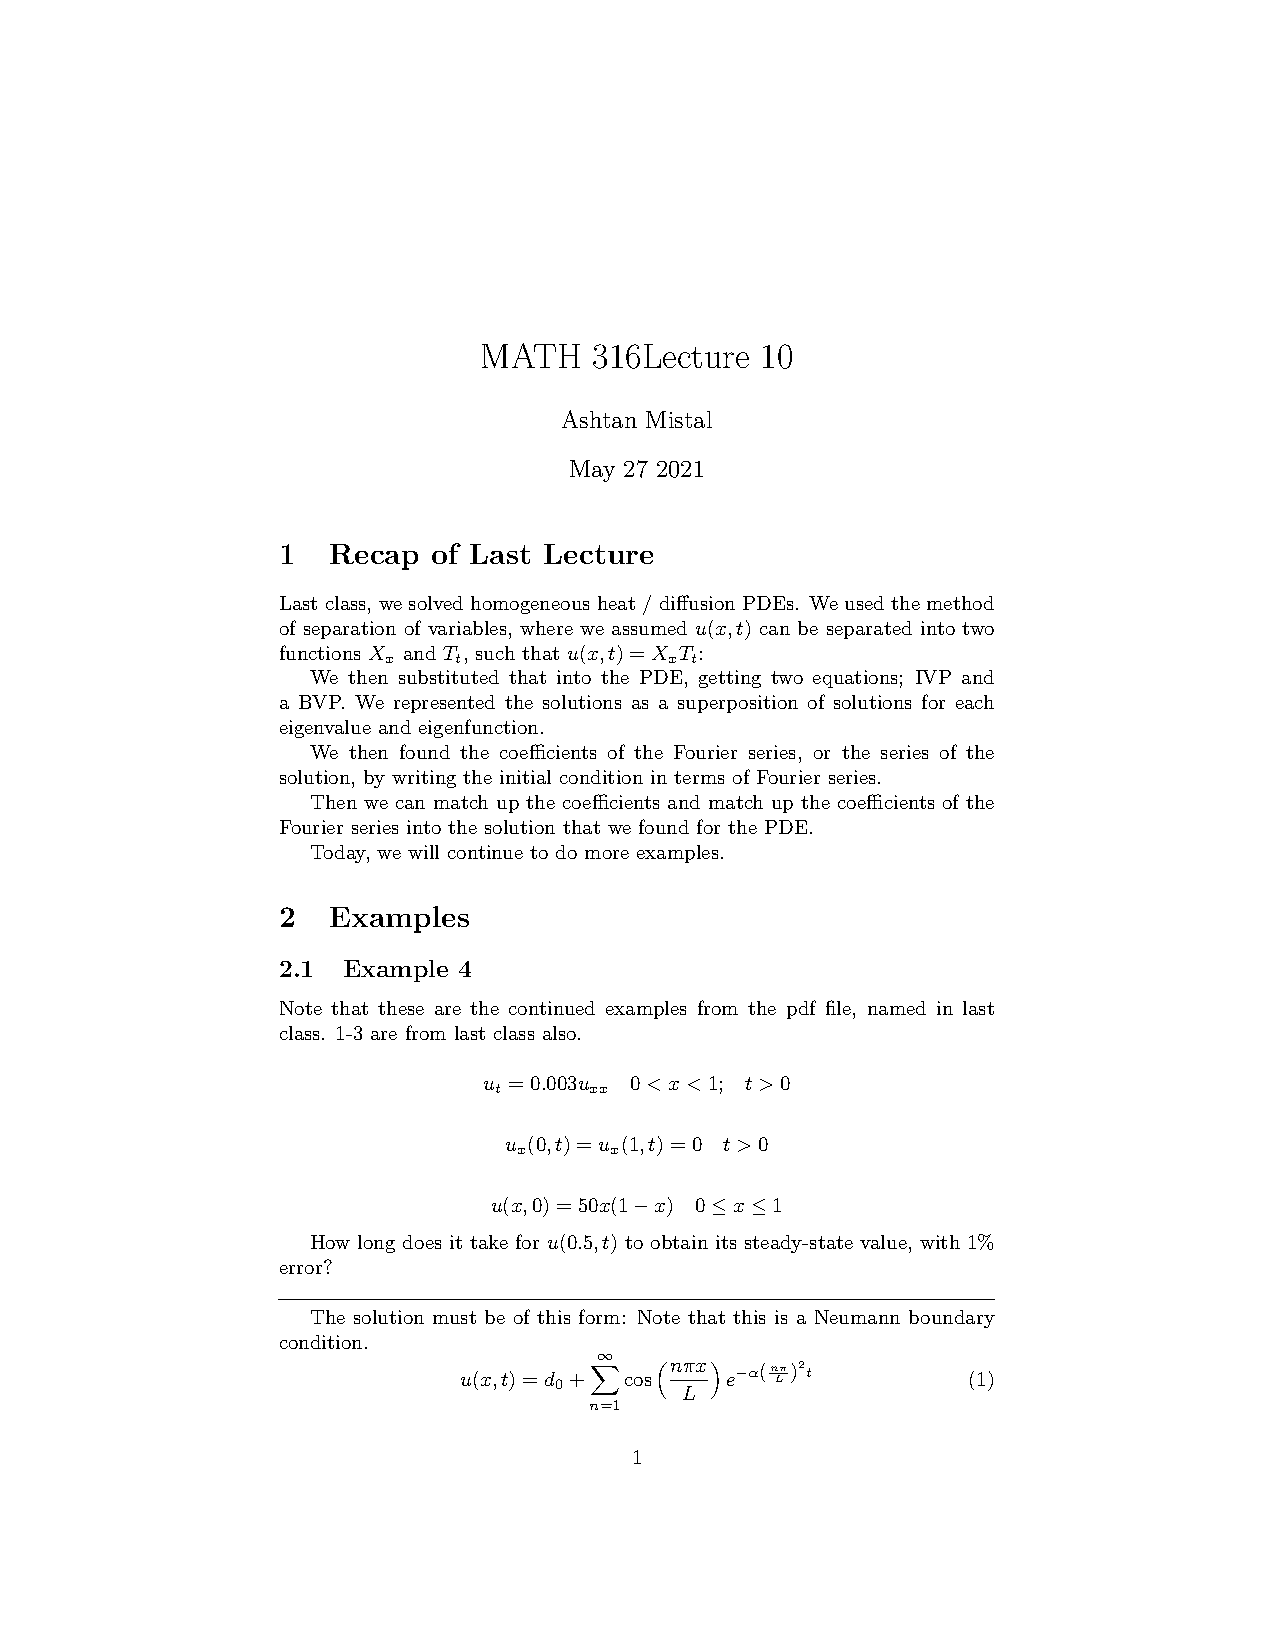
\includepdf[pages=-]{MATH 316 Lecture 10.pdf}

\chapter{Lecture 11}
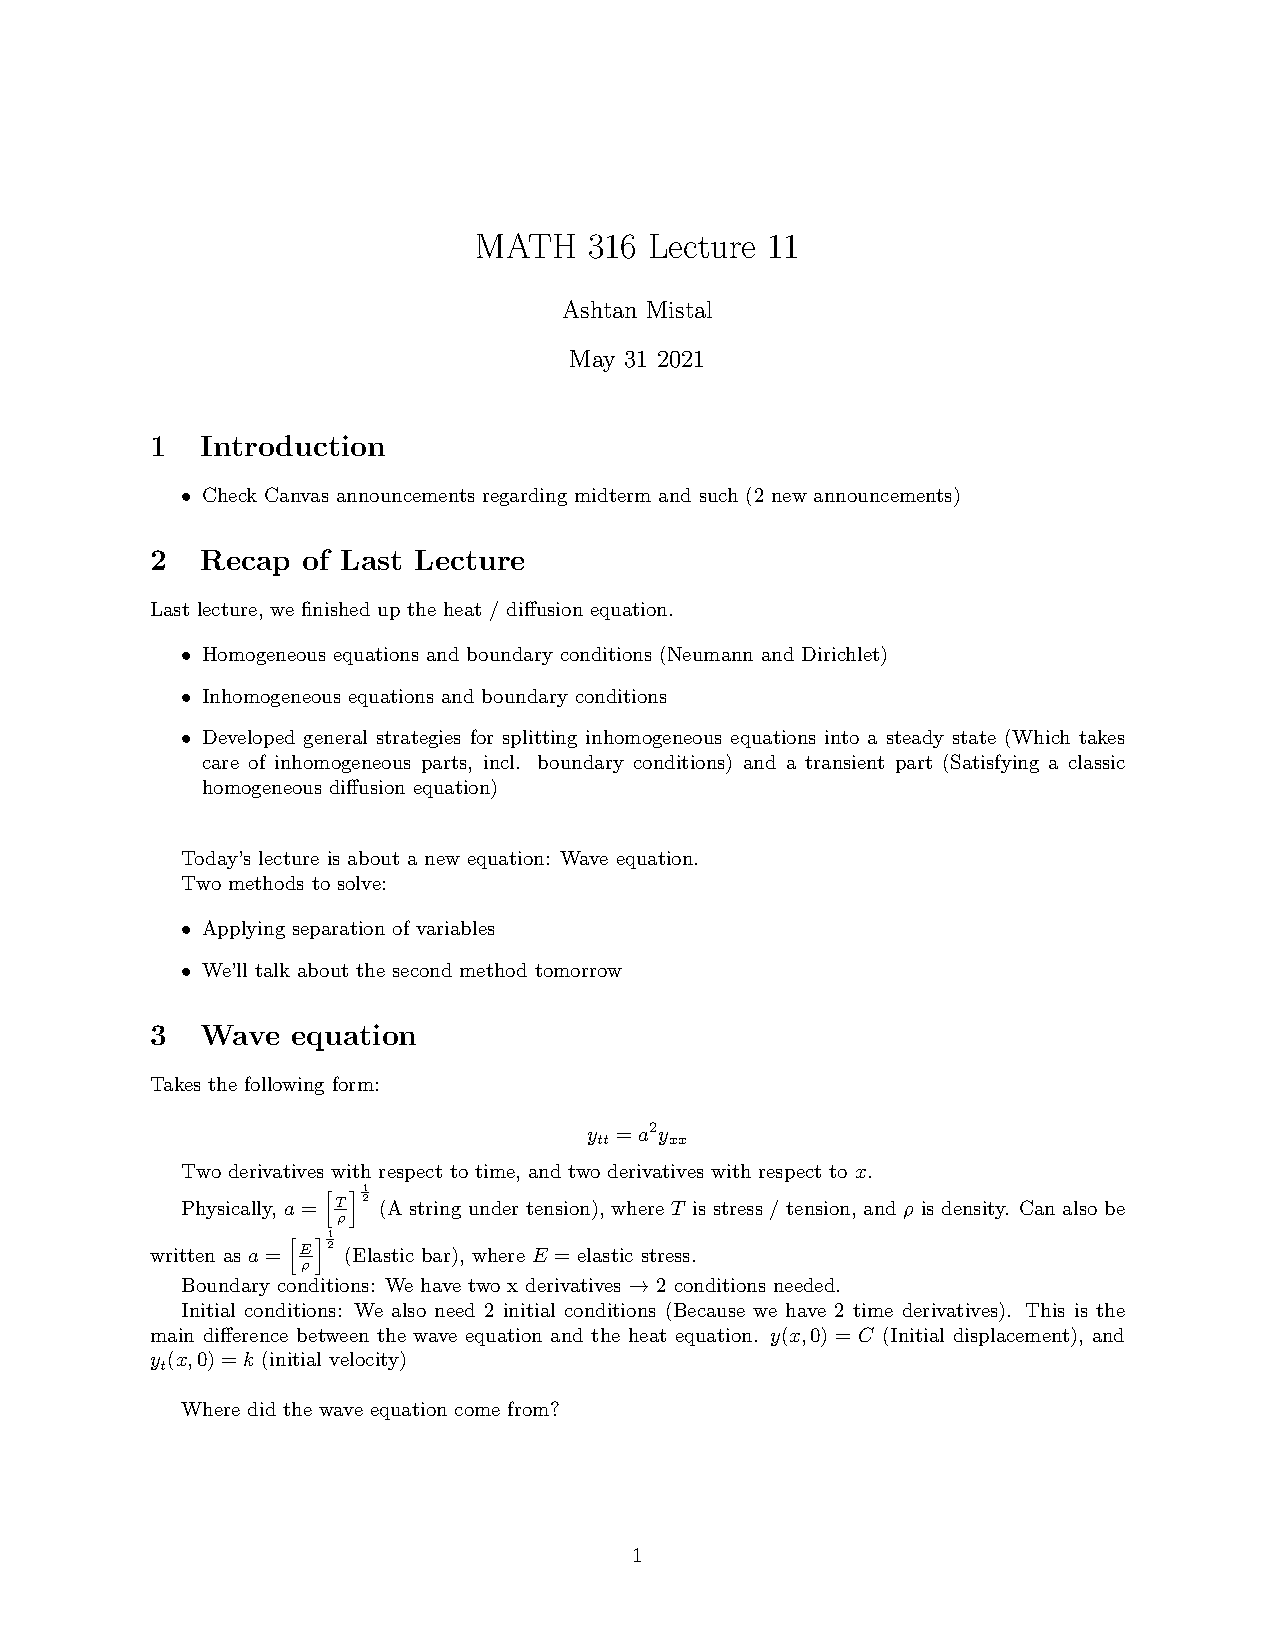
\includepdf[pages=-]{MATH 316 Lecture 11.pdf}

\chapter{Lecture 12}
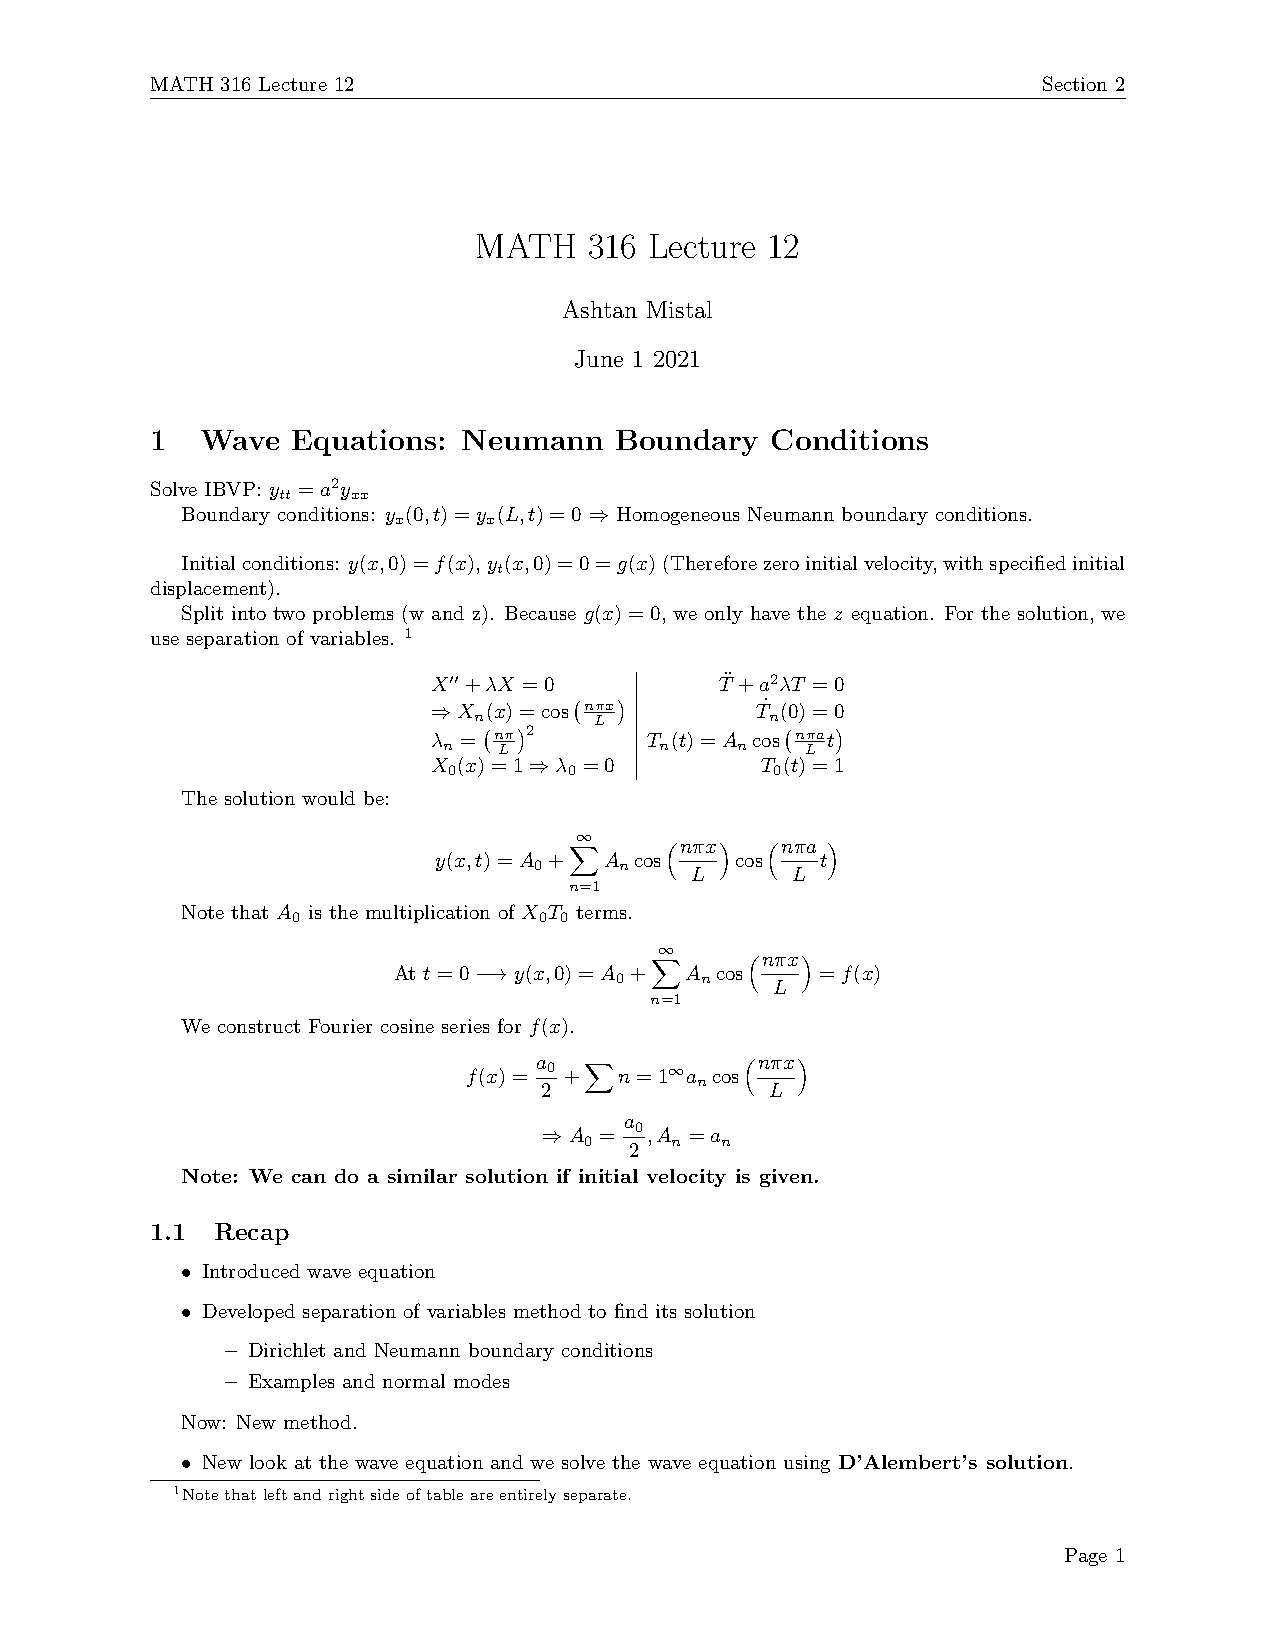
\includepdf[pages=-]{MATH 316 Lecture 12.pdf}

\end{document}
